%%% The main file. It contains definitions of basic parameters and includes all other parts.

%% Settings for single-side (simplex) printing
% Margins: left 40mm, right 25mm, top and bottom 25mm
% (but beware, LaTeX adds 1in implicitly)
\documentclass[12pt,a4paper]{report}
\setlength\textwidth{145mm}
\setlength\textheight{247mm}
\setlength\oddsidemargin{15mm}
\setlength\evensidemargin{15mm}
\setlength\topmargin{0mm}
\setlength\headsep{0mm}
\setlength\headheight{0mm}
% \openright makes the following text appear on a right-hand page
\let\openright=\clearpage

%% Settings for two-sided (duplex) printing
% \documentclass[12pt,a4paper,twoside,openright]{report}
% \setlength\textwidth{145mm}
% \setlength\textheight{247mm}
% \setlength\oddsidemargin{14.2mm}
% \setlength\evensidemargin{0mm}
% \setlength\topmargin{0mm}
% \setlength\headsep{0mm}
% \setlength\headheight{0mm}
% \let\openright=\cleardoublepage

%% Generate PDF/A-2u
\usepackage[a-2u]{pdfx}

%% Character encoding: usually latin2, cp1250 or utf8:
\usepackage[utf8]{inputenc}

%% Prefer Latin Modern fonts
\usepackage{lmodern}

%% Further useful packages (included in most LaTeX distributions)
\usepackage{amsmath}        % extensions for typesetting of math
\usepackage{amsfonts}       % math fonts
\usepackage{amsthm}         % theorems, definitions, etc.
\usepackage{amssymb}
\usepackage{bbding}         % various symbols (squares, asterisks, scissors, ...)
\usepackage{bm}             % boldface symbols (\bm)
\usepackage{graphicx}       % embedding of pictures
\usepackage{fancyvrb}       % improved verbatim environment
\usepackage{natbib}         % citation style AUTHOR (YEAR), or AUTHOR [NUMBER]
\usepackage[nottoc]{tocbibind} % makes sure that bibliography and the lists
			    % of figures/tables are included in the table
			    % of contents
\usepackage{dcolumn}        % improved alignment of table columns
\usepackage{booktabs}       % improved horizontal lines in tables
\usepackage{paralist}       % improved enumerate and itemize
\usepackage[usenames]{xcolor}  % typesetting in color

\usepackage{tikz}
\usetikzlibrary{automata}
\usetikzlibrary{positioning}
\usetikzlibrary{arrows}
\tikzset{my_automaton/.style={->,>=latex,semithick,bend angle=20}}
\tikzset{my_state/.style={circle, very thick, minimum size=0.4cm}}
\tikzset{my_named_state/.style={circle, thick, minimum size=0.7cm, inner sep=0.05cm}}
\tikzset{my_initial_state/.style={initial by arrow, initial text=}}
\tikzset{my_accepting_state/.style={accepting by double, thick}}

\usepackage{subfig}
\captionsetup{format=hang,margin=5pt}

\usepackage{etoolbox}

%% SPECIMEN
% Parts marked as SPECIMEN are used for building the example PDF.
% When the official template is generated by ./mkdist, all such parts
% are deleted, as well as all calls of \X and \XXX macros.
\def\X#1{\textcolor{red}{[#1]}}
\def\XXX#1{\par\smallskip\noindent \textcolor{red}{[#1]}}
%% NEMICEPS

%%% Basic information on the thesis

% Thesis title in English (exactly as in the formal assignment)
\def\ThesisTitle{Thesis title \X{as in the formal assignment}}

% Author of the thesis
\def\ThesisAuthor{Tomáš Svoboda}

% Year when the thesis is submitted
\def\YearSubmitted{2017}
\def\PlaceSubmitted{Prague}

% Name of the department or institute, where the work was officially assigned
% (according to the Organizational Structure of MFF UK in English,
% or a full name of a department outside MFF)
\def\Department{Department of Algebra}

% Is it a department (katedra), or an institute (ústav)?
\def\DeptType{Department}

% Thesis supervisor: name, surname and titles
\def\Supervisor{doc. Štěpán Holub, Ph.D.}

% Supervisor's department (again according to Organizational structure of MFF)
\def\SupervisorsDepartment{Department of Algebra}

% Study programme and specialization
\def\StudyProgramme{Mathematics}
\def\StudyBranch{Mathematical Methods of Information Security}

% An optional dedication: you can thank whomever you wish (your supervisor,
% consultant, a person who lent the software, etc.)
\def\Dedication{%
Dedication.
}

% Abstract (recommended length around 80-200 words; this is not a copy of your thesis assignment!)
\def\Abstract{%
Abstract. \X{Recommended length around 80--200 words. This is not a~copy of your thesis assignment!}
}

% 3 to 5 keywords (recommended), each enclosed in curly braces
\def\Keywords{%
{key} {words} \X{usually 3 to~5 key words or phrases}
}

%% The hyperref package for clickable links in PDF and also for storing
%% metadata to PDF (including the table of contents).
%% Most settings are pre-set by the pdfx package.
\hypersetup{unicode}
\hypersetup{breaklinks=true}

% Definitions of macros (see description inside)
%%% The field of all real, natural, and whole numbers
\newcommand{\R}{\mathbb{R}}
\newcommand{\N}{\mathbb{N}}
\newcommand{\Z}{\mathbb{Z}}

% Command for power set
\newcommand{\ps}[1]{\mathbb{P}(#1)}
% Command for rational expression
\newcommand{\re}[1]{{\mathsf{#1}}}
% Commands for star height and generalised star height
\newcommand{\h}[1]{{\mathsf{h}[#1]}}
\newcommand{\gh}[1]{{\mathsf{gs h}[#1]}}
% Command for automaton
\newcommand{\aut}[1]{{\mathcal{#1}}}
% Command for transition
\newcommand{\tr}[2][]{{\; \xrightarrow[#1]{\: \; #2 \: \;} \;}}


% Title page and various mandatory informational pages
\begin{document}
\include{title}

%%% A page with automatically generated table of contents of the bachelor thesis

\tableofcontents

%%% Each chapter is kept in a separate file
%\chapter*{Introduction}
\addcontentsline{toc}{chapter}{Introduction}

Kleene~\cite{Kleene56}, in result known as Kleene’s Theorem, shows that automata and expressions correspond to each other and characterise the same class of languages. Eggan~\cite{Eggan63} refines this result by defining a measure of complexity for both of them: loop complexity for automata and star height for expressions, and by showing they correspond to each other by characterising the same classes of languages. In this thesis we limit ourselves to the presentation of star height, and to the proof, due to Dejean and Schützenberger~\cite{DejeanSchutzenberger66}, which states that the star height hierarchy is infinite. They show that for any integer $k \leq 0$, there exists a~rational language of star height $k$ over two letter alphabet. We end by touching on another notion, the generalised star height, which may divide the family of rational languages into only two parts.

The determination of the star height of a~language turns out to be one of the most difficult problems in automata theory. McNaughton~\cite{McNaughton67} presented first notable result, an~algorithm for finding the star height of certain family of languages, so called \emph{pure-group languages}. Hashiguchi first~\cite{Hashiguchi1982} provided an~algorithm for deciding whether or not an~arbitrary rational language is of star height one and then~\cite{Hashiguchi1988}, after six years, an~algorithm to determine the star height of any rational language. The algorithm for the general case was not practical, being of non-\textsc{ELEMENTARY} complexity class. Kirsten~\cite{Kirsten05} devised a~more efficient algorithm than Hashiguchi's, decidable in $2^{2^{\aut{O}(n)}}$ space.
\chapter{Introduction}

In the first section we state same definitions that are considered and lay down notation that is used in the work. In the second section we provide some additional definitions and observations that are more specific to the presented problem.

\section{Basic definitions \& notation}

\begin{defn} \X{List of definitions and notation that need to be introduced:}\\
    \X{Word, factors, $|\cdot|_a$}\\
    \X{Automaton}\\
    \X{Expression, expression equivalence, star height (of expression, of language)}
\end{defn}

\section{\X{Additional definitions}}

\begin{defn}
    An automaton $\mathcal{A} = \langle Q, {\{a,b\}}^*, E, I, T \rangle$ is called \emph{ring automaton~${\mathcal{R}(n)}$}, if $I = P = \{q\}$ and there is a bijection $\varphi: \Z_n \to Q$, that
    \[
        \forall \, z \in Z_n \; \exists \: (\varphi(z),a,\varphi(z+1)), (\varphi(z),b,\varphi(z-1)) \in E.
    \]
\end{defn}

\begin{example}
    \autoref*{fig:automaton_R8} shows ring automaton~${\mathcal{R}(8)}$.
\end{example}

\begin{figure}[h]
    \centering
    \begin{tikzpicture}[my_automaton]
    \tikzstyle{every state}=[my_state]
    \tikzstyle{initial}=[my_initial_state]
    \tikzstyle{accepting}=[my_accepting_state]
    %\draw[help lines] (-1.5,1.5) grid (1.5,-1.5);
    \node[state, initial, accepting] (0) at (180:1.5) {};
    \node[state] (1) at (135:1.5) {};
    \node[state] (2) at (90:1.5) {};
    \node[state] (3) at (45:1.5) {};
    \node[state] (4) at (0:1.5) {};
    \node[state] (5) at (-45:1.5) {};
    \node[state] (6) at (-90:1.5) {};
    \node[state] (7) at (-135:1.5) {};

    \path
        (0) edge [above, bend left] node [near start, above left=-1mm] {$a$} (1)
        (1) edge [above, bend left] node [right] {$b$} (0)
        (1) edge [above, bend left] node [above] {$a$} (2)
        (2) edge [above, bend left] node [below right=-1mm] {$b$} (1)
        (2) edge [above, bend left] node [above right=-1mm] {$a$} (3)
        (3) edge [above, bend left] node [near start, below left=-1mm] {$b$} (2)
        (3) edge [above, bend left] node [right] {$a$} (4)
        (4) edge [above, bend left] node [left] {$b$} (3)
        (4) edge [above, bend left] node [right] {$a$} (5)
        (5) edge [above, bend left] node [above left=-1mm] {$b$} (4)
        (5) edge [above, bend left] node [below] {$a$} (6)
        (6) edge [above, bend left] node [above] {$b$} (5)
        (6) edge [above, bend left] node [below] {$a$} (7)
        (7) edge [above, bend left] node [above] {$b$} (6)
        (7) edge [above, bend left] node [left] {$a$} (0)
        (0) edge [above, bend left] node [above right=-1mm] {$b$} (7)
    ;
\end{tikzpicture}
    \caption{Automaton~${\mathcal{R}(8)}$}\label{fig:automaton_R8}
\end{figure}
\chapter{Eggan's question}

\cite{Eggan63} asks whether there are languages with arbitrarily large star height. In this section we present proof first due to~\cite{DejeanSchutzenberger66} and recently formulated in~\cite{Sakarovitch09}.

Throughout this chapter we use language $W_q = {\{f \mid |f|_a \equiv |f|_b \bmod 2^q \}}$.

\begin{thm}\label{thm:main}
    The language $W_q$ has star height~$q$.
\end{thm}

For the~proof we need to find an~expression of star height~$q$ denoting~$W_q$. That is done in~Lemma~\ref*{lm:expression_existence}. Then it remains to show that $W_q$ has the star height of at~least~$q$.

\begin{lemma}\label{lm:expression_existence}
    For each $q \in \N$ there is an expression of star height~$q$, that denotes~$W_q$.
\end{lemma}

\begin{proof}
    $W_q$ is recognised by an automaton~${\mathcal{R}(2^q)}$. By following a specific order~$\omega$ in the elimination method on $W_q$ we get an expression of a~star height $q$. First we set expressions
    \begin{alignat*}{5}
        X_1 = a^2 , \quad Y_1 = b^2, \quad &\text{ and } \quad Z_1 = ab + ba.
    \intertext{Then for every integer $n$ we have}
        X_{n+1} = X_n Z_n^* X_n , \quad Y_{n+1} = Y_n Z_n^* Y_n, \quad &\text{ and } \quad Z_{n+1} = Z_n + X_n Z_n^* Y_n + Y_n Z_n^* X_n.
    \end{alignat*}
    It follows that
    \[
        W_q = {(X_q + Y_q + Z_q)}^*.
    \]
    Since $X_n , Y_n , \text{ and } Z_n$ have star height~$n~-~1$, we have got an~expression denoting~$W_q$ of star height~$q$.
\end{proof}

\begin{example}
    Let us have language~$W_3$ recognised by an automaton~${\mathcal{R}(8)}$. In~\autoref*{fig:automaton_R8_state_removal_steps} we show how the~state removal algorithm finds the~expression of star height~$3$ that denotes~$W_3$. For the expression at the end of the algorithm we can see following equivalence:
    \[
        {(Z_2 + {(X_2 + Y_2)}Z_2^*{(X_2 + Y_2)})}^* = {(X_3 + Y_3 + Z_3)}^* = W_3.
    \]
\end{example}

\begin{figure}%
    \centering
    \subfloat[][]{%
        \label{fig:automaton_R8_state_removal_steps-a}%
        \input{./figures/automaton_R8_removed1}}%
    \hspace{70pt}%
    \subfloat[][]{%
        \label{fig:automaton_R8_state_removal_steps-b}%
        \begin{tikzpicture}[my_automaton]
    \tikzstyle{every state}=[my_state]
    \tikzstyle{initial}=[my_initial_state]
    \tikzstyle{accepting}=[my_accepting_state]
    %\draw[help lines] (-1.5,1.5) grid (1.5,-1.5);
    \node[state, initial, accepting] (0) at (180:1.5) {};
    \node[state] (2) at (90:1.5) {};
    \node[state] (4) at (0:1.5) {};
    \node[state] (5) at (-45:1.5) {};
    \node[state] (6) at (-90:1.5) {};
    \node[state] (7) at (-135:1.5) {};

    \path
        (0) edge [loop above, left, rotate=20] node {$ab$} ()
        (0) edge [above, bend left = 20] node [above] {$a^2$} (2)
        (2) edge [above, bend left = 20] node [near start, below=+1mm] {$b^2$} (0)
        (2) edge [loop above] node [right=+1mm] {$ab+ba$} ()
        (2) edge [above, bend left = 20] node [above right=-1mm] {$a^2$} (4)
        (4) edge [above, bend left = 20] node [below left=-1.5mm] {$b^2$} (2)
        (4) edge [loop right] node {$ba$} ()
        (4) edge [above, bend left = 20] node [right] {$a$} (5)
        (5) edge [above, bend left = 20] node [above left=-1mm] {$b$} (4)
        (5) edge [above, bend left = 20] node [below] {$a$} (6)
        (6) edge [above, bend left = 20] node [above] {$b$} (5)
        (6) edge [above, bend left = 20] node [below] {$a$} (7)
        (7) edge [above, bend left = 20] node [above] {$b$} (6)
        (7) edge [above, bend left = 20] node [left] {$a$} (0)
        (0) edge [above, bend left = 20] node [above right=-1mm] {$b$} (7)
    ;
\end{tikzpicture}}\\
    \subfloat[][]{%
        \label{fig:automaton_R8_state_removal_steps-c}%
        \begin{tikzpicture}[my_automaton]
    \tikzstyle{every state}=[my_state]
    \tikzstyle{initial}=[my_initial_state]
    \tikzstyle{accepting}=[my_accepting_state]
    %\draw[help lines] (-1.5,1.5) grid (1.5,-1.5);
    \node[state, initial, accepting] (0) at (180:1.5) {};
    \node[state] (2) at (90:1.5) {};
    \node[state] (4) at (0:1.5) {};
    \node[state] (6) at (-90:1.5) {};
    \node[state] (7) at (-135:1.5) {};

    \path
        (0) edge [loop above, left, rotate=20] node {$ab$} ()
        (0) edge [above, bend left] node [above] {$a^2$} (2)
        (2) edge [above, bend left] node [near start, below=+1mm] {$b^2$} (0)
        (2) edge [loop above] node [right=+1mm] {$ab+ba$} ()
        (2) edge [above, bend left] node [above right=-1mm] {$a^2$} (4)
        (4) edge [above, bend left] node [below left=-1.5mm] {$b^2$} (2)
        (4) edge [loop right] node {$ab+ba$} ()
        (4) edge [above, bend left] node [right] {$a^2$} (6)
        (6) edge [above, bend left] node [above] {$b^2$} (4)
        (6) edge [loop below] node [right] {$ba$} ()
        (6) edge [above, bend left] node [below] {$a$} (7)
        (7) edge [above, bend left] node [above] {$b$} (6)
        (7) edge [above, bend left] node [left] {$a$} (0)
        (0) edge [above, bend left] node [above right=-1mm] {$b$} (7)
    ;
\end{tikzpicture}}%
    \hspace{8pt}%
    \subfloat[][]{%
        \label{fig:automaton_R8_state_removal_steps-d}%
        \begin{tikzpicture}[my_automaton]
    \tikzstyle{every state}=[my_state]
    \tikzstyle{initial}=[my_initial_state]
    \tikzstyle{accepting}=[my_accepting_state]
    %\draw[help lines] (-1.5,1.5) grid (1.5,-1.5);
    \node[state, initial, accepting] (0) at (180:1.5) {};
    \node[state] (2) at (90:1.5) {};
    \node[state] (4) at (0:1.5) {};
    \node[state] (6) at (-90:1.5) {};

    \path
        (0) edge [loop above, left, rotate=20] node {$ab+ba$} ()
        (0) edge [above, bend left = 20] node [above] {$a^2$} (2)
        (2) edge [above, bend left = 20] node [near start, below=+1mm] {$b^2$} (0)
        (2) edge [loop above] node [right=+1mm] {$ab+ba$} ()
        (2) edge [above, bend left = 20] node [above right=-1mm] {$a^2$} (4)
        (4) edge [above, bend left = 20] node [below left=-1.5mm] {$b^2$} (2)
        (4) edge [loop right] node {$ab+ba$} ()
        (4) edge [above, bend left = 20] node [right] {$a^2$} (6)
        (6) edge [above, bend left = 20] node [above] {$b^2$} (4)
        (6) edge [loop below] node [right] {$ab+ba$} ()
        (6) edge [above, bend left = 20] node [below left=-1.5mm] {$a^2$} (0)
        (0) edge [above, bend left = 20] node [above right=-1.5mm] {$b^2$} (6)
    ;
\end{tikzpicture}}\\
    \subfloat[][]{%
        \label{fig:automaton_R8_state_removal_steps-e}%
        \begin{tikzpicture}[my_automaton]
    \tikzstyle{every state}=[my_state]
    \tikzstyle{initial}=[my_initial_state]
    \tikzstyle{accepting}=[my_accepting_state]
    %\draw[help lines] (-1.5,1.5) grid (1.5,-1.5);
    \node[state, initial, initial above, accepting] (0) at (180:1.5) {};
    \node[state] (4) at (0:1.5) {};
    \node[state] (6) at (-90:1.5) {};

    \path
        (0) edge [loop left] node {$ab+ba+a^2{(ab+ba)}^*b^2$} ()
        (0) edge [above, bend left = 70] node [above] {$X_2$} (4)
        (4) edge [above, bend right = 50] node [below] {$Y_2$} (0)
        (4) edge [loop right] node {$ab+ba+b^2{(ab+ba)}^*a^2$} ()
        (4) edge [above, bend left = 20] node [right] {$a^2$} (6)
        (6) edge [above, bend left = 20] node [above] {$b^2$} (4)
        (6) edge [loop below] node [right] {$ab+ba$} ()
        (6) edge [above, bend left = 20] node [below left=-1mm] {$a^2$} (0)
        (0) edge [above, bend left = 20] node [above right=-1mm] {$b^2$} (6)
    ;
\end{tikzpicture}}\\
    \subfloat[][]{%
        \label{fig:automaton_R8_state_removal_steps-e}%
        \begin{tikzpicture}[my_automaton]
    \tikzstyle{every state}=[my_state]
    \tikzstyle{initial}=[my_initial_state]
    \tikzstyle{accepting}=[my_accepting_state]
    %\draw[help lines] (-1.5,1.5) grid (1.5,-1.5);
    \node[state, initial, initial above, accepting] (0) at (180:1.5) {};
    \node[state] (4) at (0:1.5) {};

    \path
        (0) edge [loop left] node {$Z_2$} ()
        (0) edge [bend left] node [above] {$X_2 + Y_2$} (4)
        (4) edge [bend left] node [below] {$X_2 + Y_2$} (0)
        (4) edge [loop right] node {$Z_2$} ()
    ;
\end{tikzpicture}}%
    \hspace{20pt}%
    \subfloat[][]{%
        \label{fig:automaton_R8_state_removal_steps-e}%
        \begin{tikzpicture}[->,>=latex,semithick]
    \tikzstyle{every state}=[circle, very thick, minimum size=3pt]
    \tikzstyle{initial}=[initial by arrow, initial text=]
    \tikzstyle{accepting}=[accepting by arrow]
    %\draw[help lines] (-1.5,1.5) grid (1.5,-1.5);
    \node[state, initial, initial above, accepting below] (0) at (180:1.5) {};

    \path
        (0) edge [loop right] node {$Z_2 + {(X_2 + Y_2)}Z_2^*{(X_2 + Y_2)}$} ()
    ;
\end{tikzpicture}}%
    \caption{First through seventh steps of the~state removal algorithm with order~$\omega$}%
    \label{fig:automaton_R8_state_removal_steps}%
\end{figure}

\begin{proof}[Proof of \autoref*{thm:main}]
\end{proof}
\chapter{Further developments}

In the previous chapter we have shown how to calculate the star height of a particular family of languages. K. Hashiguchi gave the solution of the general case in~\cite{Hashiguchi1988}, but it was described on multiple occasions as very difficult to read. D. Kirsten presented several papers, including~\cite{Kirsten05}, with a new proof of Hashiguchi's result which seems far more intelligible.

%\include{epilog}

%%% Bibliography
\include{bibliography}

%%% Figures used in the thesis (consider if this is needed)
%\listoffigures

%%% Tables used in the thesis (consider if this is needed)
%%% In mathematical theses, it could be better to move the list of tables to the beginning of the thesis.
%\listoftables
%\XXX{In mathematical theses, it could be better to move the list of tables to the beginning of the thesis.}

%%% Abbreviations used in the thesis, if any, including their explanation
%%% In mathematical theses, it could be better to move the list of abbreviations to the beginning of the thesis.
%\chapwithtoc{List of Abbreviations}
%\XXX{In mathematical theses, it could be better to move the list of abbreviations to the beginning of the thesis.}

%%% Attachments to the bachelor thesis, if any. Each attachment must be
%%% referred to at least once from the text of the thesis. Attachments
%%% are numbered.
%%%
%%% The printed version should preferably contain attachments, which can be
%%% read (additional tables and charts, supplementary text, examples of
%%% program output, etc.). The electronic version is more suited for attachments
%%% which will likely be used in an electronic form rather than read (program
%%% source code, data files, interactive charts, etc.). Electronic attachments
%%% should be uploaded to SIS and optionally also included in the thesis on a~CD/DVD.
%%% Allowed file formats are specified in provision of the rector no. 13/2017.
%\appendix
%\chapter{Attachments}
%\XXX{Attachments to the bachelor thesis, if any. Each attachment must be referred to at least once from the text of the thesis. Attachments are numbered.}
%\XXX{The printed version should preferably contain attachments, which can be read (additional tables and charts, supplementary text, examples of program output, etc.). The electronic version is more suited for attachments which will likely be used in an electronic form rather than read (program source code, data files, interactive charts, etc.). Electronic attachments should be uploaded to SIS and optionally also included in the thesis on a~CD/DVD. Allowed file formats are specified in provision of the rector no. 13/2017.}

%\section{First Attachment}

\openright
\end{document}
